\documentclass{article}

\usepackage{graphicx}
\usepackage{amsmath}

\usepackage[margin=1in]{geometry}


\def\hwtitle{Homework template}
\def\hwauthor{Caden Gobat}
\def\hwdate{\today}

\usepackage{fancyhdr}
\lhead{\hwauthor}
\chead{\hwtitle}
\rhead{\hwdate}
\lfoot{\hwauthor}
\cfoot{}
\rfoot{\thepage}
\renewcommand{\footrulewidth}{0.4pt}
\pagestyle{fancy}

\author{\hwauthor}
\title{\hwtitle}
\date{\hwdate}

\begin{document}

\maketitle
\thispagestyle{fancy}

\section{Introduction}

It is good to start by reviewing briefly the material required for this report. 

\section{Results}

Answer each of the questions asked and comment on the significance of the results.

\bigskip
\noindent{\bf Question 1}
\medskip

The answer to this question is shown in Fig.~\ref{fig:1} ...

\begin{figure}[b]
\begin{center}
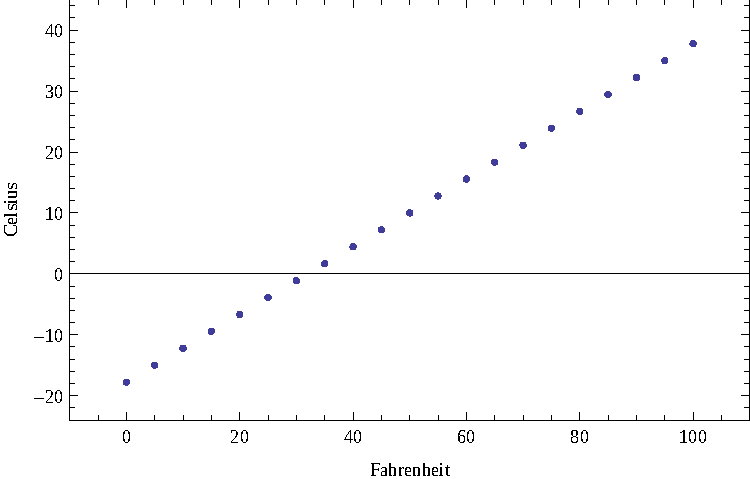
\includegraphics[width=3in]{week1proj/report/fig.pdf}
\end{center}
\caption{Use an appropriate caption for the figures included.}
\label{fig:1}
\end{figure}

\section{Conclusions}

End by summing up what you learned and what were the main challenges encountered in completing this project.

\end{document}
